\documentclass[12pt, a4paper]{article}
\usepackage{array}
\usepackage{longtable}
\usepackage[table]{xcolor}
\usepackage{hyperref}
\usepackage{float}
\usepackage[utf8]{inputenc}
\usepackage{graphicx}
\usepackage{amsmath}
\usepackage[margin=1 in]{geometry}
\usepackage{color}
\usepackage{caption}
\usepackage{pdflscape}
\usepackage{fancyhdr}

\title{Assignment 2: Foundations\\Statistical Methods for Machine Learning}
\author{Troels Thomsen - qvw203\\Rasmus Haarslev - nkh877\\Allan Martin Nielsen - jcl187}

\setlength\parindent{0pt}		% noindent through whole document
\usepackage[parfill]{parskip}	% extra linebreak on new paragraph

\begin{document}
\pagestyle{empty}
\maketitle
\pagenumbering{gobble}
\newpage

\tableofcontents
\newpage

\pagenumbering{arabic}
\pagestyle{fancy}
\fancyhead[LO,LE]{qvw203 - nkh877 - jcl187}
\fancyhead[RO, RE]{Assignment 2}

\section{II.1.1}
\begin{itemize}
	\item Standard training set accuracy: 0.86
	\item Standard test set accuracy: 0.789473684211
\end{itemize}

We notice that the test accuracy is slightly better than the one found with K-NN in the previous assignment, which was approximately 0.76.

\section{II.1.2}
\begin{itemize}
	\item Normalized training set accuracy: 0.6
	\item Normalized test set accuracy: 0.684210526316
\end{itemize}

We notice a worse result after normalization, which is not quite what we expected. We expected at least the same results, since we are normalizing with a linearly mapping.
However as shown in the figures below, the relative distance between the datapoints have changed.

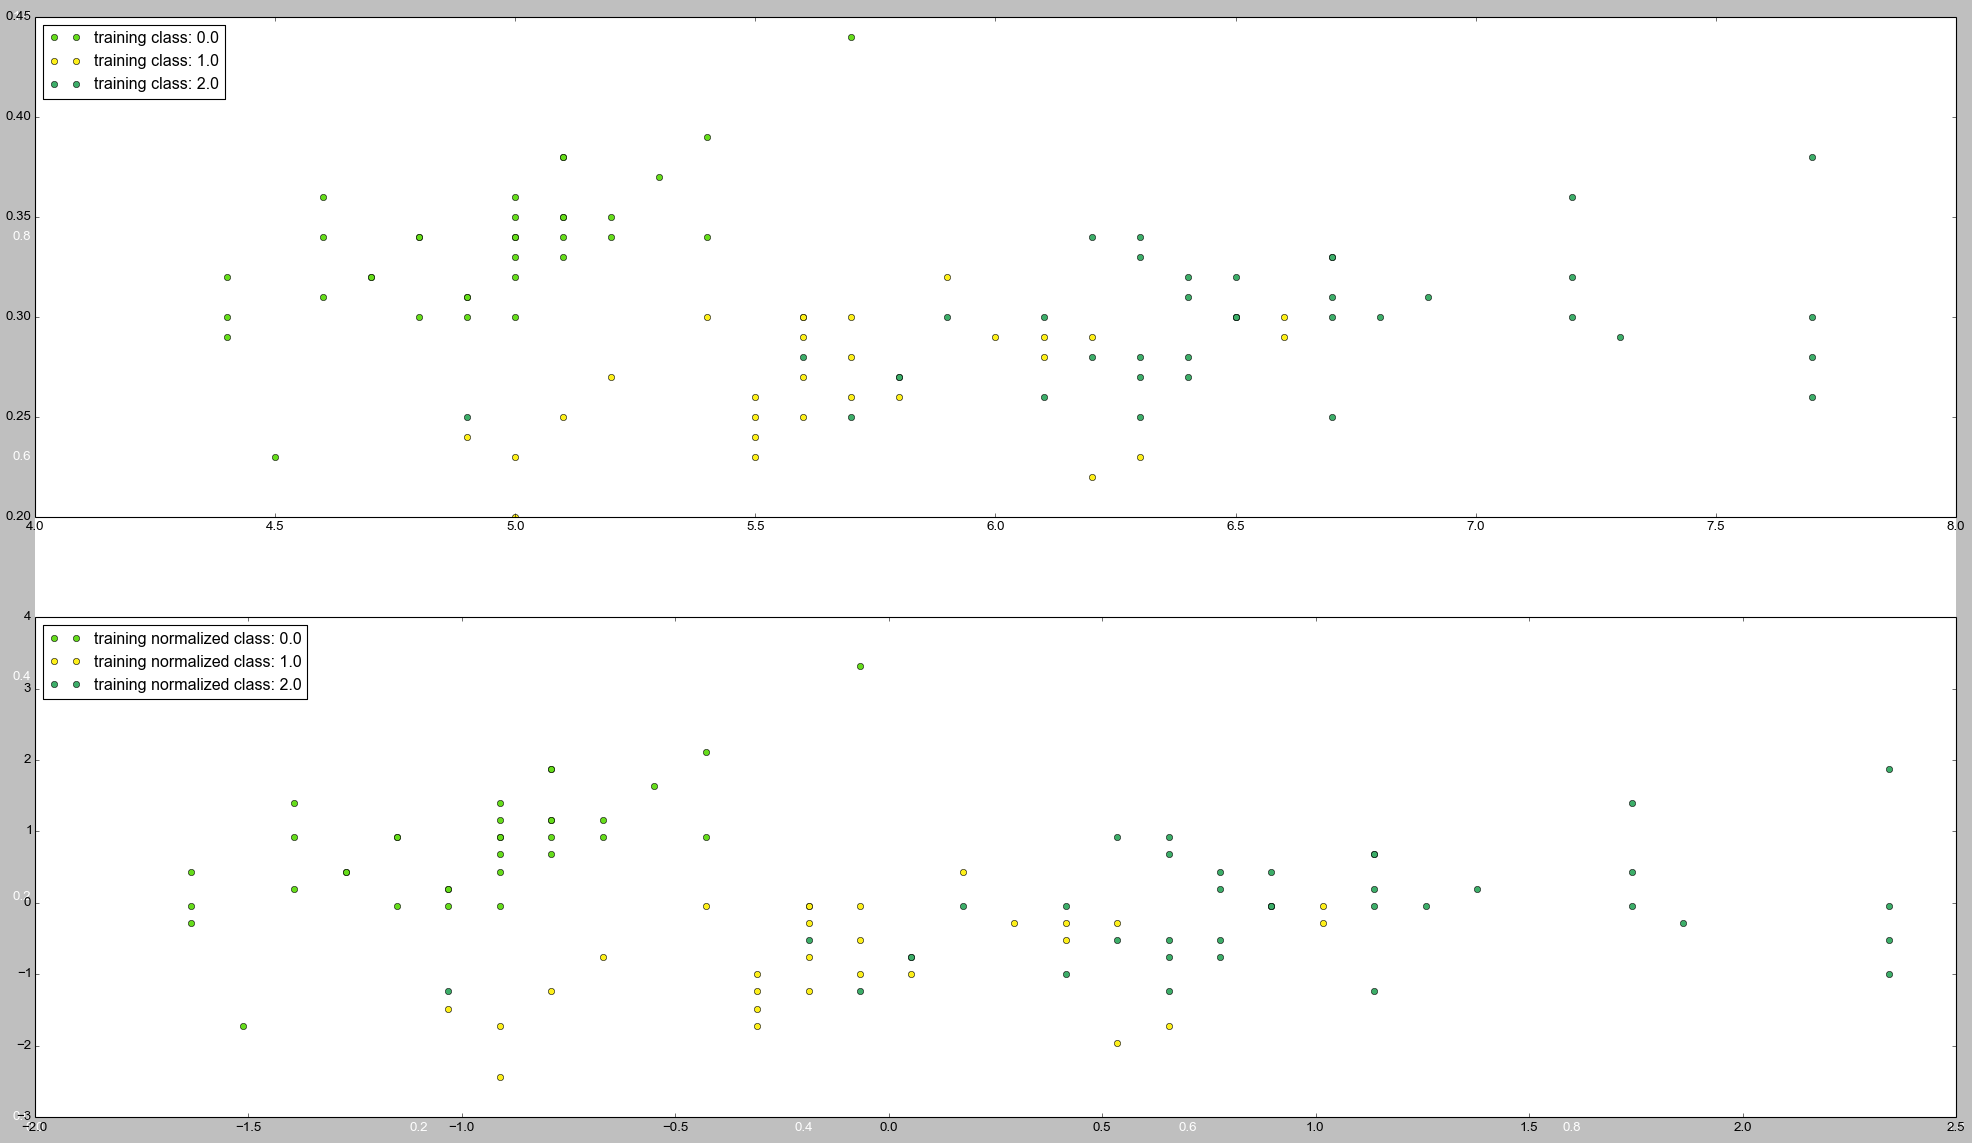
\includegraphics[scale=0.25]{lda_normalization.png}

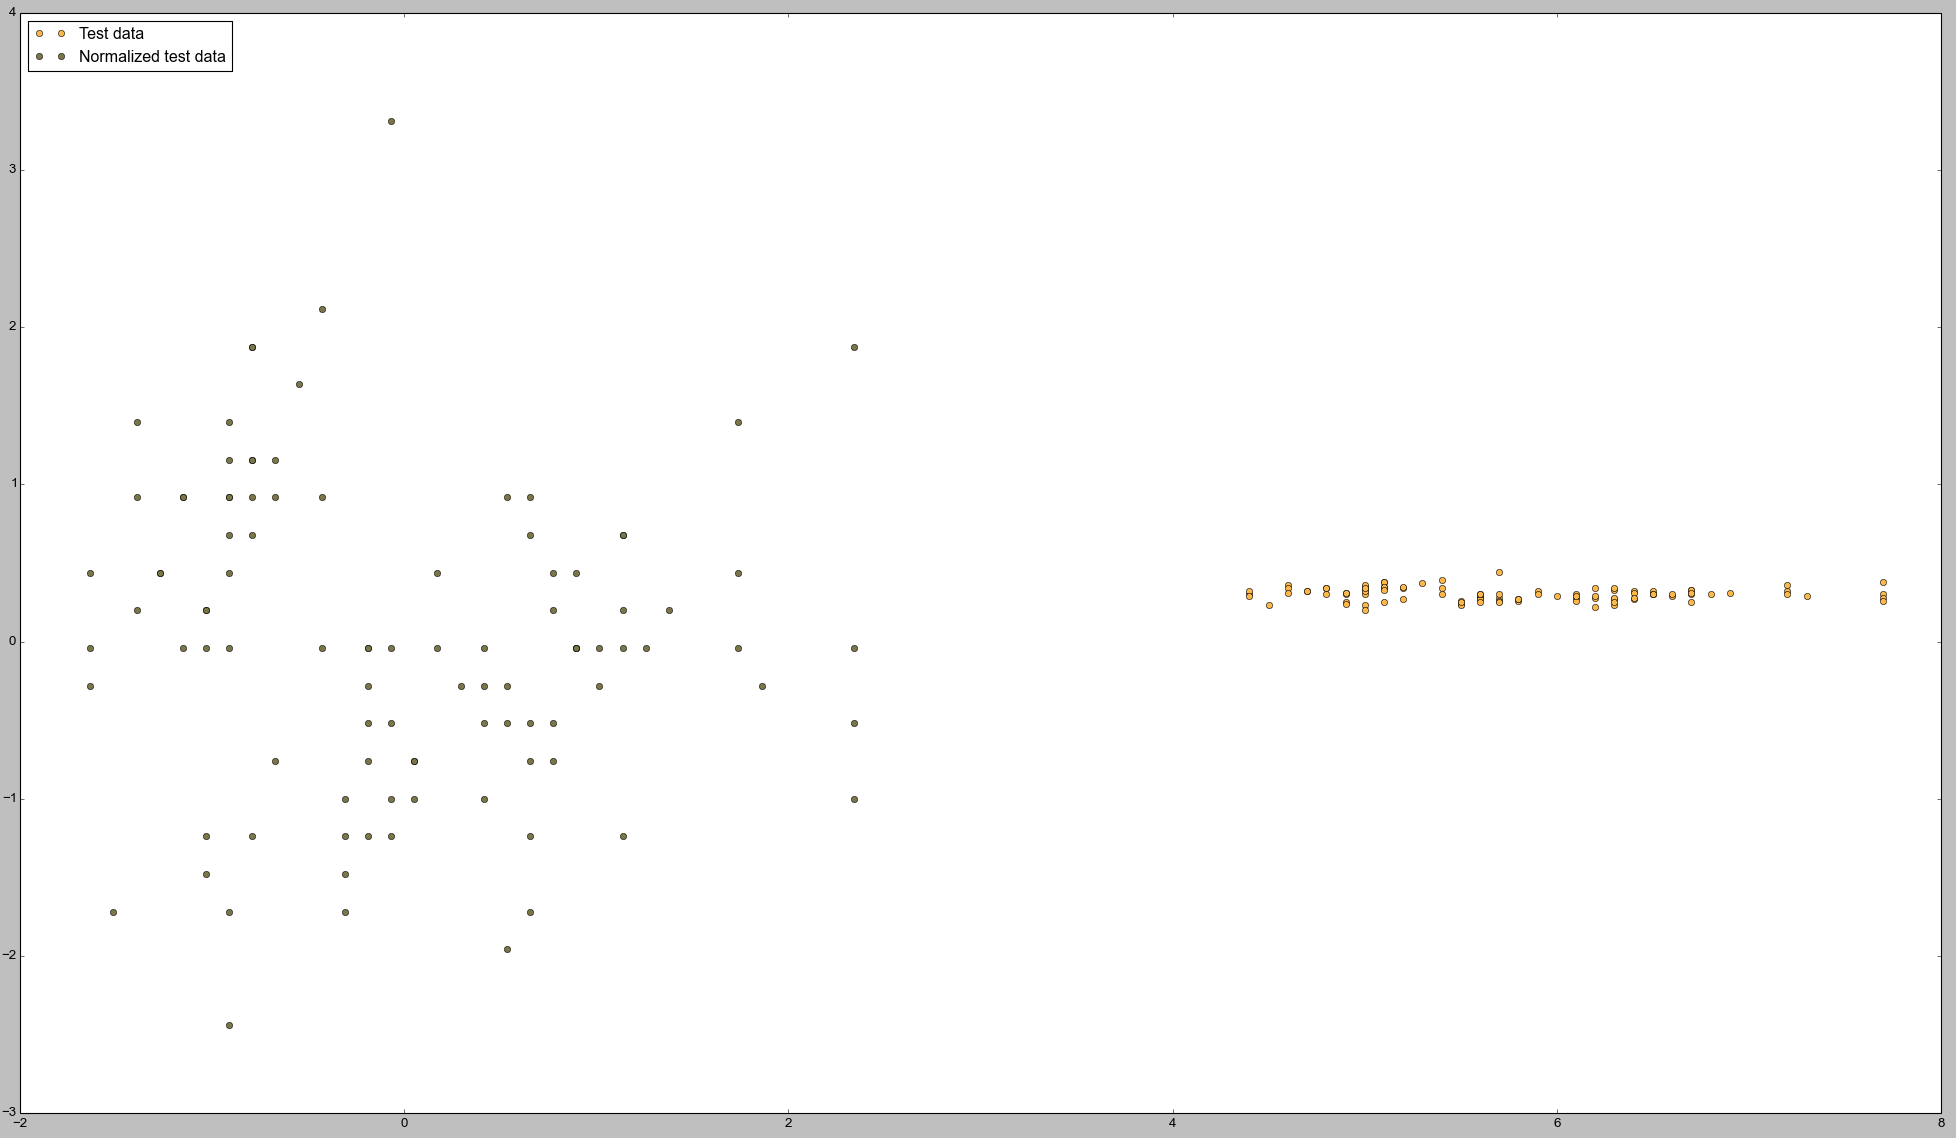
\includegraphics[scale=0.25]{lda_normalized_side.png}

This changes the covariance matrix, and since we assume identical covariance matrix for all class-conditionals, we get unpredictable results when normalizing for 0 mean and variance, before applying LDA.

\section{II.1.3}
\begin{itemize}
\item \textit{What is its (Bayes optimal) risk?}
\item \textit{What is the Bayes optimal classifier?}
\item \textit{What is the risk of the probabilistic classifier?}

We have 2 different h: $h_1(x) = 0$, and $h_2(x) = 1$. The risk of these are calculated with the risk function

\begin{eqnarray}
	\mathcal{R}_s(h = h_1) &=& \frac{1}{4} \sum^4_{i=1} (y_i - h(x_i))^2 = 0.75 \\
	\mathcal{R}_s(h = h_2) &=& \frac{1}{4} \sum^4_{i=1} (y_i - h(x_i))^2 = 0.25
\end{eqnarray}

\end{itemize}

\section{II.2.1}
\begin{itemize}
\item \textit{Which of the 3 models provide the best prediction?} 
the RMS for the three selections on the test data are as mentioned:
		\begin{itemize}
		\item \textbf{RMS Selection 1:} 29.9041602819
		\item \textbf{RMS Selection 2:} 28.6056297404
		\item \textbf{RMS Selection 3:} 17.9638970659
	\end{itemize}
\end{itemize}

\begin{figure}[H]
	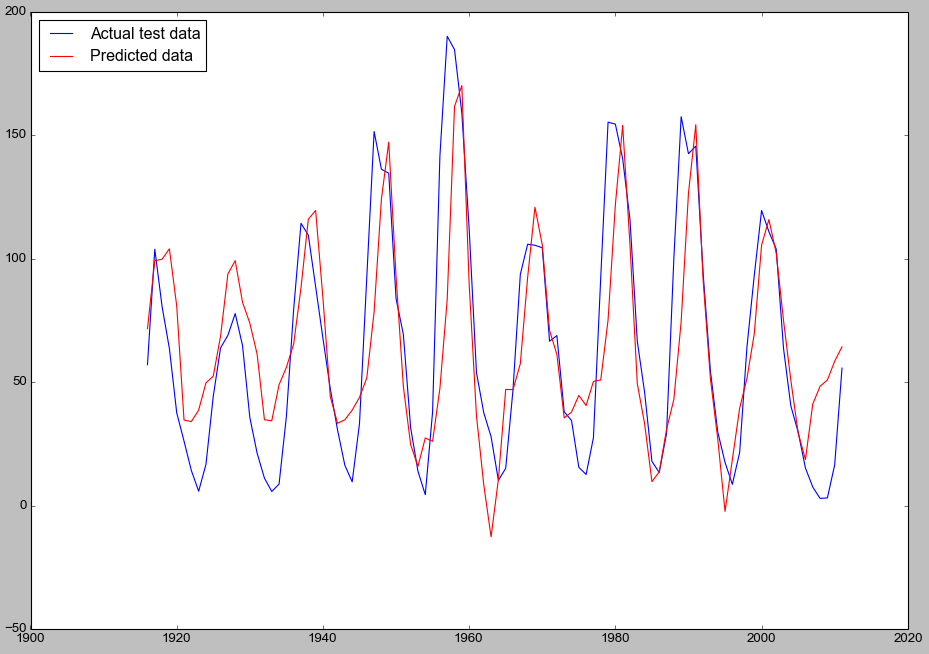
\includegraphics[scale=0.5]{ml_selection_1.png}
	\caption{Selection 1}
\end{figure}

\begin{figure}[H]
	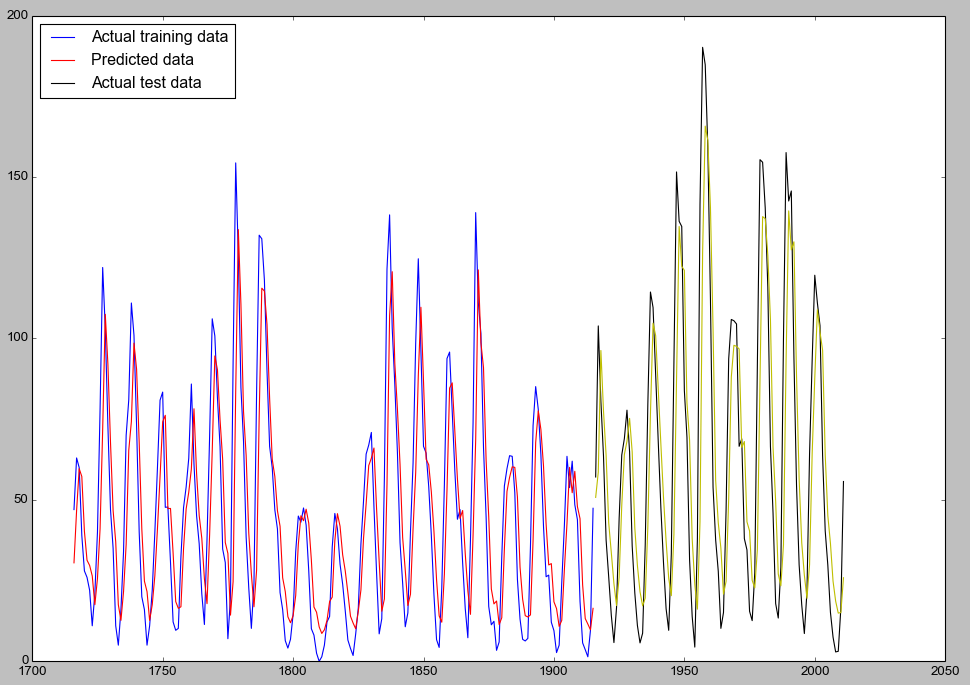
\includegraphics[scale=0.5]{ml_selection_2.png}
	\caption{Selection 2}
\end{figure}

\begin{figure}[H]
	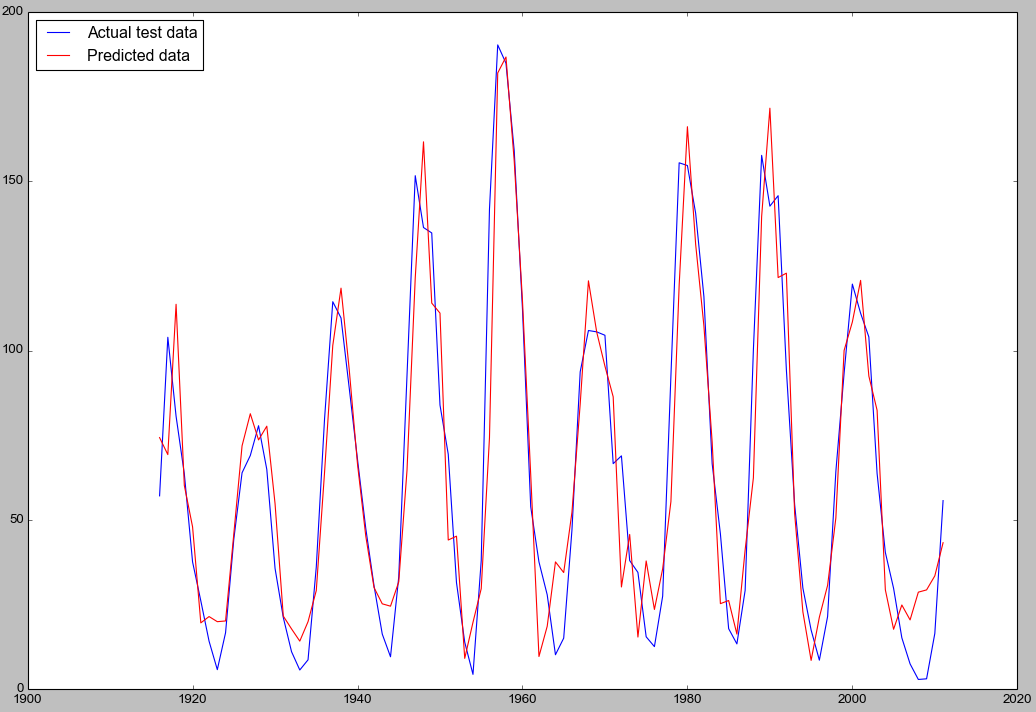
\includegraphics[scale=0.5]{ml_selection_3.png}
	\caption{Selection 3}
\end{figure}

We see from our figures that selection 3 gives the best fit on the test set, while also having the lowest RMS of 17.9638970659.

\section{II.2.2}
\begin{itemize}
\item \textit{Which of the three models seem to provide
the best prediction?}
	\begin{itemize}
		\item Like with the ML solution, the 3rd selection using the highest number of years seems to fit the best. This is confirmed by the RMS values.
	\end{itemize}
\item \textit{How do the results compare with the maximum likelihood
results?}
	These are our RMS results for $\alpha = 0.5$
	\begin{itemize}
		\item \textbf{RMS for map selection1:} 29.9112229729
		\item \textbf{RMS for map selection2:} 28.6058321345
		\item \textbf{RMS for map selection3:} 17.9664239687
	\end{itemize}
\item \textit{For what value of the prior precision parameter $\alpha$ does the RMS error go below the RMS for the maximum likelihood solution from Question II.2.1?}
	\begin{itemize}
		\item We could not find an $\alpha$ for which the RMS for MAP was lower than that found in our ML solution. As expected we came closer and closer to $RMS_{ML}$ when $\alpha$ approached 0, but as we increased $\alpha$, so did our $RMS_{MAP}$ and as such we could not improve on the results found with the ML solution.
	\end{itemize}
\end{itemize}

\section{II.2.3}
\begin{itemize}
\item \textit{Find an expression for the solution $\textbf{w}^*$ that minimizes this error function.}
\item \textit{Give two alternative interpretations of the weighted sum-of-squares
error function in terms of}
\begin{itemize}
\item[i)] \textit{data dependent noise variance}
\item[ii)] \textit{replicated data points}
\end{itemize}
\end{itemize}


\end{document}

